\chapter{Podstawy teoretyczne}

\section{Uczenie maszynowe}

Uczenie maszynowe (ang. Machine Learning) to dziedzina sztucznej inteligencji, która koncentruje się na opracowywaniu algorytmów zdolnych do automatycznego uczenia się i poprawiania wydajności na podstawie danych. W tradycyjnym programowaniu reguły określające działanie systemu są jawnie definiowane, podczas gdy w uczeniu maszynowym algorytm uczy się tych reguł na podstawie wzorców i statystyk w danych.

Uczenie maszynowe można traktować jako proces rozwiązywania problemów, w którym algorytm musi znaleźć funkcję \( f \), która przekształca dane wejściowe \( x \) na oczekiwane wyniki \( y \):

\[
	f(x) = y.
\]

Proces uczenia polega na dostosowywaniu parametrów tej funkcji, takich jak w przypadku funkcji liniowej:

\[
	f(x) = ax + b,
\]

gdzie \( a \) i \( b \) są parametrami, które algorytm dostosowuje w trakcie uczenia, aby najlepiej przybliżać dane z rzeczywistego świata.

Charakteryzacja problemów w uczeniu maszynowym obejmuje trzy główne etapy:
\begin{itemize}
	\item \textbf{Reprezentacja danych:} Jak dane są modelowane i prezentowane dla algorytmu (np. jako macierz, graf, obrazy).
	\item \textbf{Uczenie:} Proces znajdowania najlepszych parametrów modelu dla zadania na podstawie danych treningowych.
	\item \textbf{Ewaluacja:} Jak mierzy się jakość modelu na zbiorze testowym, np. poprzez dokładność, stratę, czy miary specyficzne dla problemu.
\end{itemize}

\subsection{Podział uczenia maszynowego}

Uczenie maszynowe dzieli się na trzy główne kategorie, zależnie od dostępności danych i celu uczenia:

\subsubsection{Uczenie nadzorowane (ang. Supervised Learning)}
W uczeniu nadzorowanym algorytm uczy się na zestawie danych, w którym każde wejście \( x \) ma przypisane wyjście \( y \). Celem jest zbudowanie modelu, który potrafi przewidzieć \( y \) dla nowych danych \( x \). Typowe problemy:
\begin{itemize}
	\item Klasyfikacja (np. rozpoznawanie obrazów),
	\item Regresja (np. przewidywanie cen mieszkań).
\end{itemize}
Proces ten wymaga dużej ilości danych oznaczonych i jest stosunkowo prosty do wdrożenia.

\subsubsection{Uczenie nienadzorowane (ang. Unsupervised Learning)}
W uczeniu nienadzorowanym dane treningowe nie zawierają przypisanych wyjść. Algorytm analizuje strukturę danych i szuka ukrytych wzorców. Przykładowe zastosowania:
\begin{itemize}
	\item Klasteryzacja (np. segmentacja klientów),
	\item Redukcja wymiarów (np. PCA – analiza głównych składowych).
\end{itemize}

\subsubsection{Uczenie ze wzmocnieniem (ang. Reinforcement Learning)}
Uczenie ze wzmocnieniem polega na interakcji agenta ze środowiskiem. Agent podejmuje akcje i otrzymuje nagrody, które wskazują, czy jego działanie było korzystne. Celem jest maksymalizacja długoterminowej sumy nagród. Problemy RL są bardziej złożone, ponieważ nie zawsze istnieje bezpośredni związek między akcją a natychmiastową nagrodą.

\section{Podstawowe pojęcia}

Uczenie maszynowe opiera się na kilku kluczowych pojęciach, które są fundamentem każdego modelu.

\subsection{Model}

Model w uczeniu maszynowym jest matematyczną strukturą przekształcającą dane wejściowe \(x\) na dane wyjściowe \(y\). Proces ten jest realizowany przez zestaw parametrów, które są dostosowywane w procesie uczenia w celu minimalizacji błędu predykcji.

\begin{figure}
	\begin{center}
		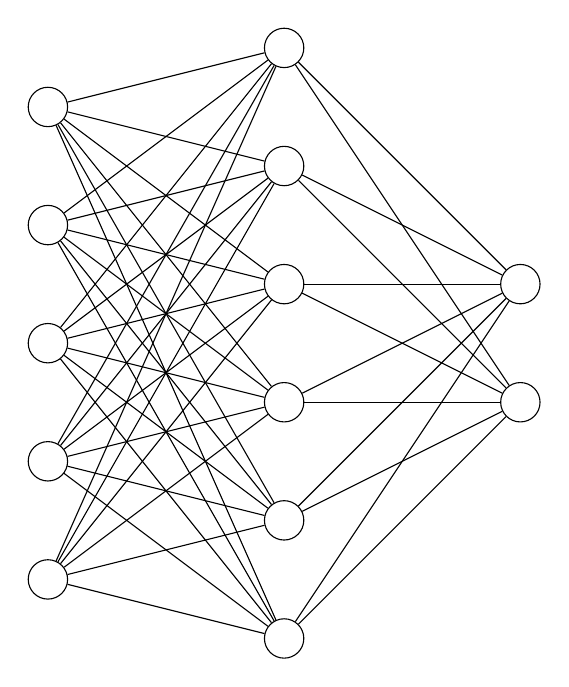
\begin{tikzpicture}
			\foreach \i in {1,...,5} {
					\node[draw, circle, minimum size=0.5cm] (L\i) at (0, -1.5*\i) {};
				}
			\foreach \i in {1,...,6} {
					\node[draw, circle, minimum size=0.5cm] (M\i) at (3, -1.5*\i+0.75) {};
				}
			\foreach \i in {1,...,2} {
					\node[draw, circle, minimum size=0.5cm] (R\i) at (6, -1.5*\i-2.25) {};
				}
			\foreach \i in {1,...,5} {
					\foreach \j in {1,...,6} {
							\draw (L\i) -- (M\j);
						}
				}
			\foreach \i in {1,...,6} {
					\foreach \j in {1,...,2} {
							\draw (M\i) -- (R\j);
						}
				}
		\end{tikzpicture}
	\end{center}
	\caption{Przykładowa wizualizacja trójwartwowej gęstej sieci neuronowej}
	\label{fig:neuron_layers}
\end{figure}

\subsubsection{Sieć neuronowa}

Sieć neuronowa jest rodzajem modelu uczenia maszynowego inspirowanym strukturą biologicznego mózgu. Składa się z neuronów ułożonych w warstwy, które przekształcają dane wejściowe na dane wyjściowe poprzez zestaw połączonych operacji matematycznych.

\paragraph{Struktura sieci:}
Sieć neuronowa składa się z:
\begin{itemize}
	\item \textbf{Warstwy wejściowej:} Przyjmuje surowe dane wejściowe.
	\item \textbf{Warstw ukrytych:} Przetwarzają dane za pomocą neuronów.
	\item \textbf{Warstwy wyjściowej:} Produkuje końcowy wynik.
\end{itemize}

\paragraph{Typy warstw:}
Różne typy warstw stosuje się w zależności od zadania. Poniżej znajduje się tabela przedstawiająca popularne typy warstw:

\begin{table}[!ht]
	\centering
	\caption{Rodzaje warstw w sieciach neuronowych}
	\label{tab:layer_types}
	\begin{center}
		\resizebox{\textwidth}{!}{
			\begin{tabular}{|c|l|}
				\hline
				\textbf{Typ warstwy}                & \textbf{Opis}                                                        \\ \hline
				Gęsta (Fully Connected)             & Każdy neuron jest połączony z każdym neuronem kolejnej warstwy.      \\ \hline
				Konwolucyjna (Convolutional Layer)  & Ekstrakcja cech lokalnych, stosowana w przetwarzaniu obrazów.        \\ \hline
				Rekurencyjna (Recurrent Layer)      & Analiza danych sekwencyjnych, np. tekstu lub szeregów czasowych.     \\ \hline
				Normalizująca (Batch Normalization) & Stabilizacja procesu uczenia poprzez normalizację wejść.             \\ \hline
				Dropout                             & Redukcja nadmiernego dopasowania przez losowe "wyłączanie" neuronów. \\ \hline
			\end{tabular}
		}
	\end{center}
\end{table}

\subsubsection{Neuron}

Neuron jest podstawową jednostką w sieci neuronowej. Otrzymuje dane wejściowe \(x\), które są przekształcane za pomocą wag \(w\) i biasu \(b\) do wartości \(z\):

\[
	z = w \cdot x + b.
\]

Wartość \(z\) jest następnie przekształcana przez funkcję aktywacyjną \(g(z)\), która nadaje sieci nieliniowość.

\subsubsection{Funkcja aktywacyjna}

Funkcja aktywacyjna jest operacją nieliniową stosowaną do wyjść neuronów. Jest kluczowa dla modelowania złożonych zależności w danych.
Może być stosowana w celu wprowadzenia nieliniowych zależności w końcowej warstwie modelu co skutkuje większymi różnicami na wyjściu modelu pomiędzy bliskimi wartościowo neuronami.

\begin{itemize}
	\item{\textbf{ReLU (Rectified Linear Unit):}
	      \[
		      g(z) = \max(0, z).
	      \]
	      \begin{figure}[!ht]
		      \centering
		      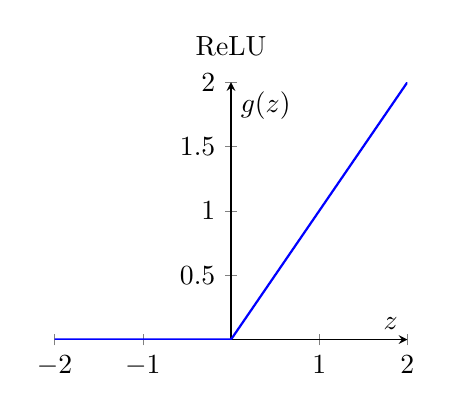
\begin{tikzpicture}
			      \begin{axis}[
					      axis lines=middle,
					      xlabel=$z$,
					      ylabel={$g(z)$},
					      title={ReLU},
					      width=0.5\textwidth,
					      height=0.4\textwidth
				      ]
				      \addplot[domain=-2:2, samples=200, thick, blue] {max(0, x)};
			      \end{axis}
		      \end{tikzpicture}
		      \caption{Funkcja aktywacyjna ReLU.}
		      \label{fig:relu}
	      \end{figure}
	      }
	\item{
	      \textbf{Sigmoid:}
	      \[
		      g(z) = \frac{1}{1 + e^{-z}}.
	      \]
	      \begin{figure}[!ht]
		      \centering
		      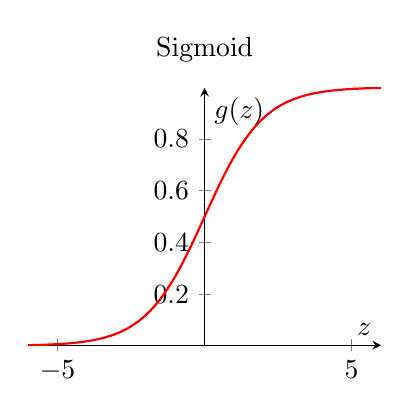
\begin{tikzpicture}
			      \begin{axis}[
					      axis lines=middle,
					      xlabel=$z$,
					      ylabel={$g(z)$},
					      title={Sigmoid},
					      width=0.5\textwidth,
					      height=0.4\textwidth
				      ]
				      \addplot[domain=-6:6, samples=200, thick, red] {1/(1 + exp(-x))};
			      \end{axis}
		      \end{tikzpicture}
		      \caption{Funkcja aktywacyjna Sigmoid.}
		      \label{fig:sigmoid}
	      \end{figure}
	      }
	\item {
	      \textbf{Tanh:}
	      \[
		      g(z) = \tanh(z) = \frac{e^z - e^{-z}}{e^z + e^{-z}}.
	      \]

	      \begin{figure}[!ht]
		      \centering
		      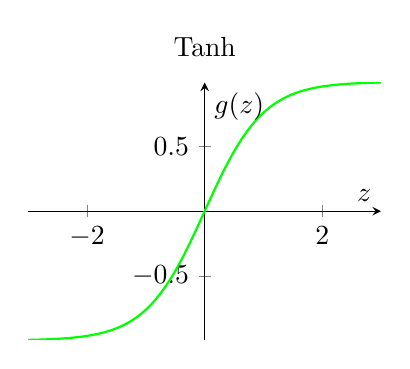
\begin{tikzpicture}
			      \begin{axis}[
					      axis lines=middle,
					      xlabel=$z$,
					      ylabel={$g(z)$},
					      title={Tanh},
					      width=0.5\textwidth,
					      height=0.4\textwidth
				      ]
				      \addplot[domain=-3:3, samples=200, thick, green] {tanh(x)};
			      \end{axis}
		      \end{tikzpicture}
		      \caption{Funkcja aktywacyjna Tanh.}
		      \label{fig:tanh}
	      \end{figure}
	      }
\end{itemize}

\subsubsection{Parametry modelu}

Parametry modelu (np. wagi \(w\) i biasy \(b\)) są wartościami liczbowymi, które model dostosowuje podczas procesu uczenia. Trenowanie modelu polega na minimalizacji funkcji kosztu (ang. loss function), która mierzy różnicę między przewidywaniami modelu a rzeczywistymi wartościami.

%TODO
%\[
%	L = \frac{1}{n} \sum_{i=1}^{n} (y_i - \hat{y}_i)^2,
%\]

gdzie \(y_i\) to rzeczywista wartość, a \(\hat{y}_i\) to przewidywana wartość modelu.

\subsection{Środowisko}
Środowisko jest otoczeniem, w którym agent działa. Dostarcza stanów \( S \), które opisują aktualną sytuację, oraz nagród \( R \), które oceniają jakość podjętych działań.

\begin{itemize}
	\item \textbf{Symulowane gry i światy wirtualne:}
	      \begin{itemize}
		      \item Atari Games (ALE) \cite{BELLEMARE2013}: Gry 8-bitowe, takie jak \textit{Breakout}, \textit{Pong} czy \textit{Space Invaders}.
		      \item Super Mario Bros \cite{KARPATHY2015}: Gra platformowa, w której agent uczy się przechodzić poziomy, omijając przeszkody i eliminując przeciwników.
		      \item OpenAI Gym \cite{BROCKMAN2016}: Zbiór środowisk do testowania algorytmów uczenia ze wzmocnieniem, w tym proste gry i symulacje.
		      \item VizDoom \cite{KEMPKA2016}: Gra FPS (First Person Shooter), gdzie agent eksploruje trójwymiarowe środowisko i uczy się strategii przetrwania.
	      \end{itemize}

	\item \textbf{Środowiska robotyczne:}
	      \begin{itemize}
		      \item MuJoCo \cite{TODOROV2012}: Symulacje robotów do testowania algorytmów sterowania.
		      \item Roboschool \cite{SCHULMAN2017}: Środowiska do trenowania robotów w zadaniach, takich jak chodzenie czy chwytanie obiektów.
		      \item PyBullet \cite{COUMANS2016}: Otwarte środowisko do symulacji fizyki, używane do modelowania zachowań robotów.
	      \end{itemize}

	\item \textbf{Symulacje rzeczywistego świata:}
	      \begin{itemize}
		      \item Autonomous Driving (Carla) \cite{DOSOVITSKIY2017}: Symulacje jazdy autonomicznej.
	      \end{itemize}

	\item \textbf{Środowiska edukacyjne:}
	      \begin{itemize}
		      \item Maze Solvers \cite{SUTTON2018}: Symulacje labiryntów, w których agent uczy się znajdować wyjście.
		      \item GridWorld \cite{RUSSELL2003}: Proste środowisko siatki 2D, gdzie agent uczy się optymalnej strategii poruszania.
	      \end{itemize}
\end{itemize}

\subsection{Stan}

Stan (ang. State) jest kluczowym elementem w uczeniu ze wzmocnieniem, który opisuje bieżącą sytuację w środowisku. Stan zawiera wszystkie istotne informacje potrzebne agentowi do podejmowania decyzji, takich jak pozycja w przestrzeni, otoczenie, zasoby czy inne dane kontekstowe. Formalnie, stan w danym momencie \( t \) oznaczamy jako \( s_t \).

\paragraph{Definicja stanu:}
Stan powinien być na tyle kompletny, aby agent mógł na jego podstawie przewidzieć konsekwencje swoich działań. W praktyce oznacza to, że stan \( s_t \) powinien być wystarczający do określenia następnego stanu \( s_{t+1} \), jeśli znana jest akcja \( a_t \) podjęta przez agenta.

\paragraph{Przykłady stanów w różnych środowiskach:}
Stany mogą przyjmować różne formy w zależności od charakteru środowiska:
\begin{itemize}
	\item \textbf{Gry komputerowe:} W grach wideo stan może obejmować pozycję postaci, punkty życia, liczbę przeciwników oraz przeszkody na planszy. Na przykład w grze Super Mario Bros stan \( s_t \) może zawierać:
	      \begin{itemize}
		      \item Pozycję postaci Mario (\texttt{mario\_x}, \texttt{mario\_y}),
		      \item Liczbę pozostałych żyć,
		      \item Czas do zakończenia poziomu.
	      \end{itemize}
	      Źródło: \cite{BELLEMARE2013, KARPATHY2015}.

	\item \textbf{Robotyka:} W robotyce stan może zawierać:
	      \begin{itemize}
		      \item Kąt wychylenia ramienia robota,
		      \item Pozycję chwytaka,
		      \item Siły oddziałujące na czujniki.
	      \end{itemize}
	      Źródło: \cite{TODOROV2012, SCHULMAN2017}.

	\item \textbf{Autonomiczne pojazdy:} W symulacjach jazdy autonomicznej stan może obejmować:
	      \begin{itemize}
		      \item Pozycję pojazdu względem pasa ruchu,
		      \item Prędkość i przyspieszenie,
		      \item Pozycję innych pojazdów oraz sygnalizację świetlną.
	      \end{itemize}
	      Źródło: \cite{DOSOVITSKIY2017}.
\end{itemize}

\paragraph{Reprezentacja stanu:}
Stan może być reprezentowany w różnych formatach w zależności od charakteru środowiska:
\begin{itemize}
	\item Wartości liczbowe (np. pozycja na planszy),
	\item Macierze (np. obrazy w grach komputerowych),
	\item Grafy (np. w symulacjach sieci społecznych lub ruchu drogowego).
\end{itemize}

\paragraph{Wymagania wobec stanu:}
Aby algorytm mógł skutecznie działać, stan powinien być:
\begin{itemize}
	\item \textbf{Dostępny:} Agent musi być w stanie zaobserwować stan \( s_t \) w każdym kroku czasowym \( t \).
	\item \textbf{Markowski:} Stan \( s_t \) musi być kompletny, tj. zawierać wszystkie informacje potrzebne do określenia przyszłości na podstawie bieżących akcji (\emph{Markov Decision Process}\cite{PUTERMAN1994}).
\end{itemize}

\paragraph{Znaczenie stanu w uczeniu ze wzmocnieniem:}
Dokładne określenie stanu jest kluczowe dla skuteczności algorytmu. Niekompletny lub zbyt uproszczony stan może prowadzić do nieoptymalnych decyzji agenta, natomiast nadmiarowa ilość informacji w stanie zwiększa złożoność obliczeniową algorytmu.

\paragraph{Wpływ na złożoność obliczeniową:}
Ilość parametrów modelu (wagi i biasy) rośnie wraz z liczbą połączeń neuronów. W przypadku wielowarstwowych sieci neuronowych liczba parametrów gwałtownie wzrasta, co prowadzi do większych wymagań obliczeniowych i pamięciowych. Dla warstwy gęstej (ang. fully connected) liczba parametrów \(P\) jest określana jako:

\[
	P = (n_{\text{input}} \cdot n_{\text{output}}) + n_{\text{output}},
\]

gdzie:
\begin{itemize}
	\item \(n_{\text{input}}\) – liczba neuronów wejściowych,
	\item \(n_{\text{output}}\) – liczba neuronów wyjściowych,
	\item \(n_{\text{output}}\) dodatkowo uwzględnia biasy.
\end{itemize}

Zwiększanie liczby warstw i neuronów pozwala na modelowanie bardziej złożonych funkcji, ale także zwiększa ryzyko nadmiernego dopasowania (ang. overfitting) oraz wydłuża czas trenowania modelu. Optymalizacja liczby parametrów jest kluczowa dla zachowania równowagi między dokładnością modelu a jego efektywnością obliczeniową.

\subsection{Akcja}

Akcja (ang. Action) to decyzja podejmowana przez agenta w danym stanie środowiska. Określa, jak agent wpływa na otoczenie, prowadząc do zmiany stanu i potencjalnego otrzymania nagrody. Zbiór wszystkich możliwych akcji agenta nazywa się przestrzenią akcji \(A\).

\paragraph{Typy przestrzeni akcji:}
\begin{itemize}
	\item \textbf{Skończona (ang. Discrete):} Agent wybiera spośród ograniczonej liczby akcji, np. ruch w lewo, w prawo, skok.
	\item \textbf{Ciągła (ang. Continuous):} Agent wybiera wartość z określonego przedziału, np. prędkość czy kąt obrotu.
\end{itemize}

\paragraph{Przykłady akcji:}
\begin{itemize}
	\item Ruch przestrzenny, np. zmiana pozycji w labiryncie.
	\item Manipulacja obiektami, np. podnoszenie lub przesuwanie przedmiotów.
	\item Regulacja parametrów, np. ustawianie prędkości w pojazdach autonomicznych.
\end{itemize}

Każda akcja prowadzi do zmiany stanu środowiska \(s_t\) na \(s_{t+1}\), zgodnie z funkcją przejścia \(P(s_{t+1} | s_t, a_t)\). Wybór akcji jest określany przez strategię (ang. policy), która może być deterministyczna lub stochastyczna.

\subsection{Nagroda}

Nagroda (ang. Reward) to wartość liczbowa, którą agent otrzymuje po wykonaniu akcji w danym stanie. Jest kluczowym elementem w uczeniu ze wzmocnieniem, ponieważ kieruje zachowaniem agenta, motywując go do podejmowania działań prowadzących do maksymalizacji długoterminowych korzyści. Nagroda w danym kroku czasowym \(t\) oznaczana jest jako \(r_t\).

\paragraph{Dobór funkcji nagrody:}
Projektowanie funkcji nagrody wymaga ostrożności, ponieważ niewłaściwy dobór może prowadzić do niepożądanego zachowania agenta. Dobrze zaprojektowana funkcja nagrody powinna:
\begin{itemize}
	\item Być zgodna z celem środowiska (np. szybkie ukończenie zadania, minimalizacja kosztów).
	\item Karać za niepożądane działania (np. kolizje w robotyce, utratę życia w grze).
	\item Oferować natychmiastową informację zwrotną, aby przyspieszyć proces uczenia.
\end{itemize}

\paragraph{Normalizacja nagrody:}
Normalizacja nagrody polega na skalowaniu wartości \(r_t\) do określonego zakresu, np. \([-1, 1]\), co zapobiega dominacji ekstremalnych wartości nad procesem uczenia. Może to również pomóc w stabilizacji algorytmu i przyspieszeniu zbieżności. Typowe metody normalizacji to:
\begin{itemize}
	\item \textbf{Z-score normalization:} Skalowanie względem średniej i odchylenia standardowego:
	      \[
		      r_t' = \frac{r_t - \mu_r}{\sigma_r},
	      \]
	      gdzie \(\mu_r\) i \(\sigma_r\) są odpowiednio średnią i odchyleniem standardowym nagród.
	\item \textbf{Min-max scaling:} Skalowanie do określonego zakresu:
	      \[
		      r_t' = \frac{r_t - \min(r)}{\max(r) - \min(r)}.
	      \]
\end{itemize}

\paragraph{Przykłady nagród:}
\begin{itemize}
	\item W grach komputerowych: zdobycie punktów, przejście na kolejny poziom, kara za utratę życia \cite{BELLEMARE2013}.
	\item W robotyce: nagroda za poprawne uchwycenie przedmiotu lub utrzymanie równowagi \cite{TODOROV2012}.
	\item W pojazdach autonomicznych: nagroda za płynne poruszanie się po drodze, kara za kolizje \cite{DOSOVITSKIY2017}.
\end{itemize}

\subsection{Funkcja kosztu (Loss)}

Funkcja kosztu jest kluczowym elementem procesu uczenia modelu, ponieważ określa, jak bardzo bieżące predykcje modelu różnią się od wartości docelowych. W przypadku uczenia ze wzmocnieniem (ang. Reinforcement Learning), funkcja kosztu jest związana z różnicą pomiędzy bieżącymi wartościami \(Q(s, a)\) a wartościami docelowymi wyznaczonymi na podstawie nagród i przewidywań przyszłych stanów.

\paragraph{Znaczenie funkcji kosztu:}
\begin{itemize}
	\item \textbf{Minimalizacja różnic:} Funkcja kosztu prowadzi do optymalizacji parametrów modelu \(\theta\), minimalizując różnice pomiędzy bieżącymi wartościami \(Q(s, a)\) a wartościami docelowymi.
	\item \textbf{Stabilność procesu uczenia:} Wprowadzenie sieci docelowej \(\theta^{-}\) pozwala na bardziej stabilne obliczanie wartości docelowych \(y_t\), co zapobiega niestabilności procesu uczenia wynikającej z dynamicznie zmieniających się wartości \(Q(s, a)\).
	\item \textbf{Wrażliwość na parametry:} Funkcja kosztu jest wrażliwa na odpowiedni dobór współczynnika dyskontowego \(\gamma\) i strategii aktualizacji sieci docelowej, co wpływa na szybkość i jakość uczenia.
\end{itemize}

\section{Double Q-Learning}

Double Q-Learning to zaawansowany algorytm uczenia ze wzmocnieniem, będący rozszerzeniem klasycznego Q-Learningu. Jego głównym celem jest redukcja przeszacowania wartości akcji, co jest typowym problemem w tradycyjnym Q-Learningu. W tej sekcji omówione zostaną podstawy algorytmu Q-Learning, problem przeszacowania, struktura Double Q-Learning oraz jego zastosowania.

\subsection{Podstawy Q-Learning}

Q-Learning jest jednym z najbardziej znanych algorytmów uczenia ze wzmocnieniem, który pozwala agentowi uczyć się optymalnej strategii działania w środowisku poprzez iteracyjne aktualizowanie funkcji wartości \(Q(s, a)\). Funkcja ta ocenia korzyść z podjęcia określonej akcji \(a\) w stanie \(s\).

Równanie aktualizacji w klasycznym Q-Learningu opiera się na równaniu Bellmana:

\[
	Q(s, a) \leftarrow Q(s, a) + \alpha \left( r + \gamma \max_{a'} Q(s', a') - Q(s, a) \right),
\]

gdzie:
\begin{itemize}
	\item \(s\) – aktualny stan,
	\item \(a\) – podjęta akcja,
	\item \(r\) – nagroda za wykonanie akcji \(a\),
	\item \(s'\) – następny stan po wykonaniu akcji \(a\),
	\item \(\alpha\) – współczynnik uczenia, kontrolujący szybkość aktualizacji,
	\item \(\gamma\) – współczynnik dyskontowy, określający znaczenie przyszłych nagród.
\end{itemize}

Celem algorytmu Q-Learning jest iteracyjne zbliżanie wartości funkcji \(Q(s, a)\) do jej optymalnych wartości \(Q^*(s, a)\). Wartość \(Q^*(s, a)\) reprezentuje maksymalną sumę oczekiwanych nagród, jaką agent może uzyskać, rozpoczynając w stanie \(s\), wykonując akcję \(a\), a następnie postępując zgodnie z najlepszą możliwą strategią.

\subsection{Problem przeszacowania wartości}

W Q-Learningu akcje są wybierane na podstawie maksymalnej wartości \(Q(s, a)\). Jednak proces aktualizacji również wykorzystuje tę maksymalną wartość, co prowadzi do przeszacowania wyników, szczególnie w środowiskach o dużej zmienności. Problem przeszacowania wynika z faktu, że maksymalizowanie wartości \(Q(s, a)\) na etapie wyboru i aktualizacji wprowadza błędy, które się kumulują.

\subsection{Double Q-Learning: Struktura i działanie}

Double Q-Learning rozwiązuje problem przeszacowania, wprowadzając dwie oddzielne funkcje wartości, \(Q_1\) i \(Q_2\). Te funkcje są aktualizowane naprzemiennie, co pozwala na rozdzielenie procesu wyboru akcji od procesu aktualizacji wartości.

\paragraph{Równania aktualizacji:}
W danym kroku czasowym \(t\):
\begin{itemize}
	\item Jeśli aktualizowana jest funkcja \(Q_1\), proces przebiega według wzoru:
	      \[
		      Q_1(s, a) \leftarrow Q_1(s, a) + \alpha \left( r + \gamma Q_2(s', \arg\max_{a'} Q_1(s', a')) - Q_1(s, a) \right),
	      \]
	\item Jeśli aktualizowana jest funkcja \(Q_2\), proces przebiega według wzoru:
	      \[
		      Q_2(s, a) \leftarrow Q_2(s, a) + \alpha \left( r + \gamma Q_1(s', \arg\max_{a'} Q_2(s', a')) - Q_2(s, a) \right).
	      \]
\end{itemize}

Rozdzielenie aktualizacji między \(Q_1\) i \(Q_2\) pozwala na bardziej precyzyjne oszacowanie wartości \(Q(s, a)\), ponieważ wybór akcji opiera się na jednej funkcji, a aktualizacja na drugiej.

\paragraph{Strategia \(\epsilon\)-greedy}

Strategia \(\epsilon\)-greedy (ang. \(\epsilon\)-greedy policy) to jedna z najczęściej stosowanych metod równoważenia eksploracji i eksploatacji w uczeniu ze wzmocnieniem. Celem tej strategii jest umożliwienie agentowi eksploracji środowiska (odkrywanie nowych akcji) przy jednoczesnym wykorzystywaniu najlepszych dotychczasowych decyzji.

W strategii \(\epsilon\)-greedy agent wybiera akcję w następujący sposób:
\begin{itemize}
	\item Z prawdopodobieństwem \(1 - \epsilon\) wybiera akcję o najwyższej wartości \(Q(s, a)\), czyli eksploatuje dotychczasową wiedzę.
	\item Z prawdopodobieństwem \(\epsilon\) wybiera losową akcję, eksplorując nowe możliwości.
\end{itemize}

Parametr \(\epsilon \in [0, 1]\) kontroluje równowagę między eksploracją a eksploatacją:
\begin{itemize}
	\item Dla \(\epsilon = 0\) agent zawsze wybiera akcję o maksymalnej wartości \(Q(s, a)\), całkowicie eksploatując swoją wiedzę.
	\item Dla \(\epsilon = 1\) agent zawsze wybiera losową akcję, skupiając się wyłącznie na eksploracji.
\end{itemize}

Często stosuje się harmonogram zmiany wartości \(\epsilon\) w czasie, tzw. \textit{annealing}, gdzie \(\epsilon\) początkowo jest wysokie (intensywna eksploracja), a następnie maleje w miarę zdobywania przez agenta wiedzy o środowisku. Dzięki temu na początku agent może zbierać informacje o środowisku, a później optymalizować swoje działania na podstawie dotychczasowych doświadczeń.

\paragraph{Model online i model docelowy}

W Double Q-Learning algorytm opiera się na rozdzieleniu funkcji wartości \(Q\) na dwie oddzielne funkcje: model online i model docelowy (ang. target model). Takie podejście pozwala na większą stabilność uczenia i bardziej precyzyjne oszacowanie wartości \(Q(s, a)\).

\begin{itemize}
	\item \textbf{Model online:} Jest to główny model używany do podejmowania decyzji przez agenta. Na podstawie modelu online agent wybiera akcje w danym stanie \(s\), kierując się strategią \( \epsilon\)-greedy lub inną strategią eksploracyjno-eksploatacyjną.
	\item \textbf{Model docelowy (target model):} Służy do aktualizacji wartości docelowych w procesie uczenia. Model docelowy jest kopią modelu online, aktualizowaną w regularnych odstępach czasu, co zapobiega nadmiernym oscylacjom wartości \(Q\) i poprawia stabilność algorytmu.
\end{itemize}

Aktualizacja wartości \(Q\) w Double Q-Learning wykorzystuje obydwa modele:
\begin{itemize}
	\item Model online wybiera najlepszą akcję w stanie \(s'\), tj. \(\arg\max_{a'} Q_\text{online}(s', a')\).
	\item Model docelowy dostarcza wartość \(Q\) dla wybranej akcji:
	      \[
		      Q_\text{target}(s, a) \leftarrow r + \gamma Q_\text{online}(s', \arg\max_{a'} Q_\text{target}(s', a')).
	      \]
\end{itemize}

Rozdzielenie wyboru akcji i ich aktualizacji na dwa modele redukuje ryzyko przeszacowania, ponieważ proces wyboru akcji i oceny ich wartości odbywa się w niezależnych kopiach funkcji \(Q\).

\subsection{Funkcja kosztu w Double Q-Learning:}

Dla algorytmu Double Q-Learning, funkcja kosztu jest definiowana jako błąd średniokwadratowy (ang. Mean Squared Error, MSE) pomiędzy wartością docelową \(y_t\) a bieżącą wartością \(Q(s_t, a_t)\):
\[
	L(\theta) = \mathbb{E}_{s_t, a_t, r_t, s_{t+1}} \left[ \left( y_t - Q(s_t, a_t; \theta) \right)^2 \right],
\]
gdzie:
\begin{itemize}
	\item \(y_t = r_t + \gamma Q(s_{t+1}, \arg\max_a Q(s_{t+1}, a; \theta); \theta^{-})\) – wartość docelowa wyznaczona przy użyciu sieci docelowej \(\theta^{-}\).
	\item \(\gamma\) – współczynnik dyskontowy, który określa wpływ przyszłych nagród.
	\item \(r_t\) – nagroda uzyskana w bieżącym kroku.
\end{itemize}

\subsection{Zalety Double Q-Learning}

Double Q-Learning ma kilka istotnych zalet w porównaniu z klasycznym Q-Learningiem:
\begin{itemize}
	\item \textbf{Redukcja przeszacowania:} Rozdzielenie procesu wyboru i aktualizacji wartości zmniejsza ryzyko błędów wynikających z nadmiernej optymistycznej oceny.
	\item \textbf{Lepsza stabilność:} Algorytm działa bardziej przewidywalnie w środowiskach o dużej zmienności lub hałasie.
	\item \textbf{Elastyczność:} Double Q-Learning można łatwo rozszerzyć na bardziej złożone algorytmy, takie jak Deep Q-Learning.
\end{itemize}
